

\subsection{Description de l'expérience}
\textbf{Description de l'expérience réalisée, méthodologie et métriques d'évaluation.} \\
It is clear that standard supervised training does not specify that the chosen loss function be resistant to adversarial examples. This has to be encoded in some way during the training process. In this section, we will perform two kinds of adversarial training on a simple network (maxout) to improve its robustness. First we add the adversarial loss to the loss function. As described in the paper, his form is as follows :
$$ f_{adv}(\theta,x,y) = \alpha f(\theta,x,y) +(1-\alpha )f(\theta,x+\epsilon sign(\nabla_{x}f(\theta,x,y),y) $$
As in the paper, we take $\alpha$ always as 0.5. Its role is similar to an effective regularizer. This means that we will constantly update the adversarial sample in our training. We generate adversarial samples at the end of each batch and calculate the losses caused by them. After that we use the obtained new losses to compute the gradient and propagate.

In the second approach, first we will train a model without adversarial training. Then, we generate the corresponding adversarial samples and add these samples to the training set. We use this training set with the adversarial samples to re-train our model. This approach is similar to data augmentation.

%\lipsum[4]

\subsection{Résultats}
\textbf{Présentation des résultats expérimentaux obtenus et  comparaison par rapport à ceux de l’article de réference.} \\
In this section, we repeat the experiments in the paper and compare the results obtained with those in the original paper. In the first adversarial training we found a significant increase in training time because the number of samples in each batch is doubled in this approach. However, we did not achieve the same results on the test set. First, in the maxout network paper, the authors achieved an accuracy of 99.06 $\%$ using the simple structure of MLP+maxout+dropout. However, in the github code given by the authors, dropout is not used and the final accuracy is only 97.3$\%$. The best accuracy we have found in other replications is 98.5$\%$. Our accuracy is 98.4$\%$ after fifty epochs, which is similar to Maxime Vandegar. By using eraly stopping, we had an average error rates without of 1.35 $\%$ and the best error rate of 1.26 $\%$, which are better than error rates without adversarial training (1.7$\%$).

\newpage
After confirming that the adversarial regular term improves the performance of the model on the original training set, we investigate whether the model is robust to adversarial samples. The results are shown in the figure below :

\begin{figure}[htbp]
\centering
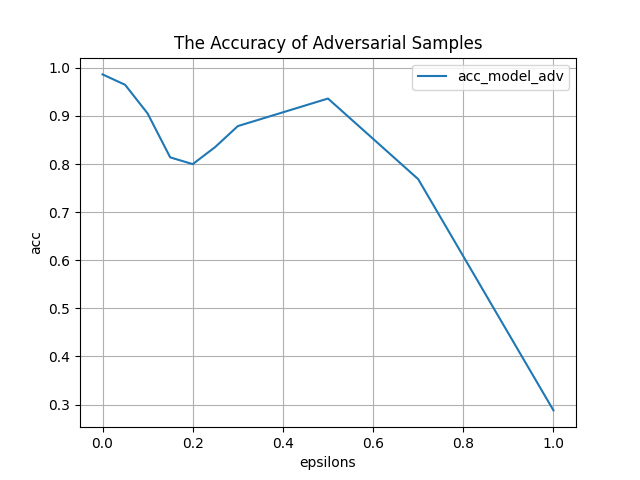
\includegraphics[width=9cm]{acc_advtraining_2.png}
\caption{Accuracy of model with adversarial training}
\end{figure}
%\lipsum[5]
We reduced the error rate from 89.4$\%$ to 19.6$\%$, which is the highest error with $\epsilon = 0.2$ for all perturbations imperceptible to humans ($\epsilon < 0.5$).
\subsection{Discussion}

\textbf{Discussion critique à partir des
résultats obtenus} \\

%\lipsum[6]


